\chapter{Results}
\label{chapter:Results}

This chapter provides the results of the performed experiments. The first section focuses on the results obtained on a simulated environment using two tasks from the Meta-World benchmark \cite{metaworld}. Here, the contribution of R-CIdL is measured by comparing its performance to that of D-COACH for different conditions of replay buffer size $K$, parameter $e$ and type of state (absolute or relative positions).
Finally, the results of two planar manipulation tasks are shown to validate R-CIdL on a real setup.



\section{Results of simulated tasks}
\label{section:results_metaworld}

To evaluate the contribution of R-CIdL with respect to the baseline method D-COACH, we did experiments with a simulated teacher on the Meta-World tasks plate-slide-v2 and drawer-open-v2  presented in sections \ref{subsection:metaworld-hockey-task} and
\ref{subsection:metaworld-open-drawer-task} respectively. 

Running some initial experiments it was observed that the type of state has an important influence on the performance of the agents. For both tasks the state consists on the coordinates in the Cartesian axes of the end effector, the coordinates of the object and the coordinates of the goal position. In the case of the plate-slide-v2 task, the object refers to the puck whereas for the drawer-open-v2 task, the object is the handle of the drawer.
If the positions of the state are absolute, the state is then equal to $[[xyz_\text{end effector}], [xyz_\text{object}], [xyz_\text{goal}]]$ 
On the other hand, if the positions are relative, then the state is equal to $[[xyz_\text{object} - xyz_\text{end effector}], [xyz_\text{goal} - xyz_\text{object}]]$. In this last case when the positions are relative to each other, not only the number of dimensions decreases but it is easier for the neural network to generalize the task.

The results for both tasks are divide in two parts. The first one shows how robust is the proposed method R-CIdL to variations of the parameters $e$ and replay buffer size $K$ in comparison to D-COACH when the state is formed by relative positions. Once the best combination of $e$ and $K$ is obtained for both methods, the experiments are repeated with those same conditions but this time the agent learns with states formed by absolute positions. The parameters used for the policy and the human model are shown in table \ref{tab:hyperparameters}. Trainings are 75000 time steps long which is approximately equivalent to 15 minutes of simulated time as the MuJoco time step duration is 0.0125 seconds.

In order to evaluate the robustness of R-CIdL, three values of $e$ and three values of $K$ are chosen. For $e$, we chose 0.01, 0.1 and 1 as these values are within the range tried during the real experiments. The three sizes for the replay buffer are 3000, 15000 and 30000; The reason behind these values is that the simulated teacher sends about 30000 corrections signals, therefore these sizes correspond to 10\%, 50\%  and 100\% of the maximum average accumulated corrections at the end of the trainings. The plots in the next subsections show the average success per episode of 20 trainings where each policy is evaluated 5 times.



\subsection{Performance of task plate-slide-v2}
\label{subsection:Performance of task plate_slide_v2}




Figure \ref{fig:results_plate_slide_buffer_e} shows the average success per episode for the task plate-slide-v2 for different values of $e$ and buffer size when the positions are relative. There are three main conclusions that can be extracted. First, R-CIdl is overall much more robust to changes in both $e$ and buffer size $K$ and it is able to reach 100\% success around minute 6. Regarding D-COACH, $e$ is the parameter that has more influence being its worst performance when $e=0.01$. And regarding the buffer size $K$, the biggest buffer is the most detrimental and the smallest results in the best performance at the end of the training.
This was expected as in D-COACH the buffer contains information gathered by all the previous old versions of the policy that may not be useful for updating the current version of the policy.


 \begin{figure}[htpb]
  \centering
  \subfloat{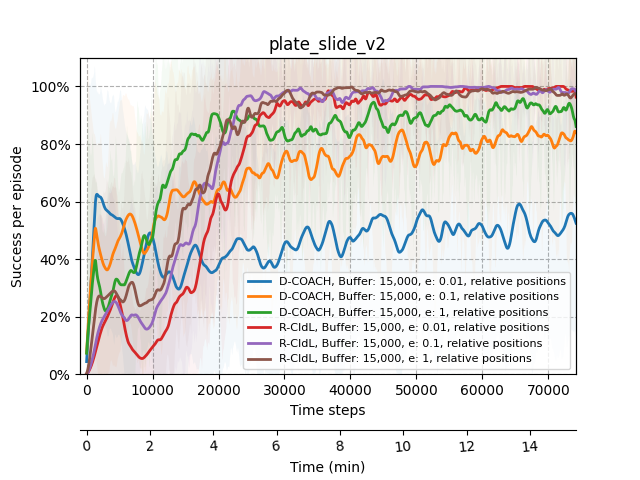
\includegraphics[width=0.5\textwidth]{figures/hockey_same_buffer_v2.png}\label{fig:plate_slide_same_buffer}}
   \hfill
  \subfloat{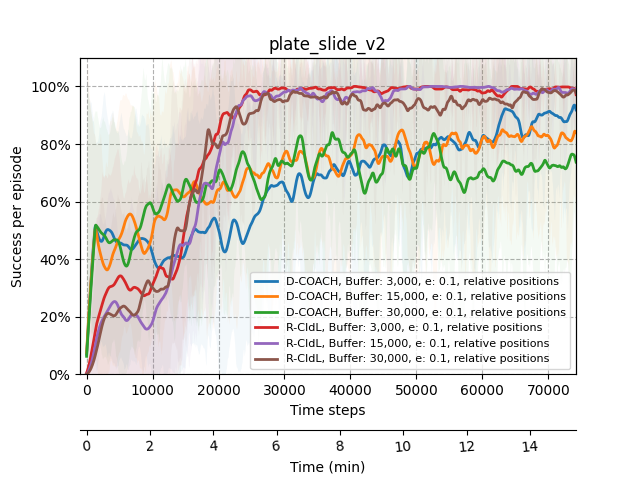
\includegraphics[width=0.5\textwidth]{figures/hockey_same_e_v2.png}\label{fig:plate_slide_same_e}}
  \caption{plate-slide-v2 results using a simulated teacher $P_h: \alpha = 0.9; \tau =  0.000015$. On the left, a comparison of the influence of the $e$ parameter on the baseline method D-COACH and on R-CIdL. On the right, a comparison of how different buffer sizes $K$ affect both methods.}
  \label{fig:results_plate_slide_buffer_e}
\end{figure}


      
From the previous analysis, the best combinations of buffer size $K$ and $e$ for both methods when positions are relative are $K=30000$ and $e=0.1$ for R-CIdL and $K=15000$ and $e=1$ for D-COACH. The experiments are repeated with the same values but this time considering absolute positions instead of relative ones. Figure \ref{fig:results_plate_slide_best} shows this comparison where R-CIdL, it is able to reach similar levels of performance as in the case of relative positions whereas the performance of D-COACH decreases a 20\%.



\begin{figure}[H]
    \centering
    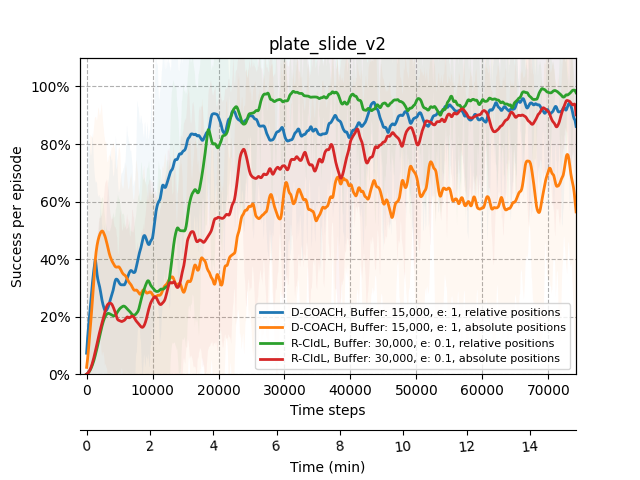
\includegraphics[width=.60\textwidth]{figures/hockey_best_v2.png}
    \caption{plate-slide-v2 results using a simulated teacher $P_h: \alpha = 0.9; \tau =  0.000015$. Comparison of the best performance of each method in relative positions, against their performances in absolute positions with the same conditions of $K$ and $e$.}
    \label{fig:results_plate_slide_best}
\end{figure}

\subsection{Performance of task drawer\_open\_v2}
\label{subsection:Performance of task drawer_open_v2}

Similar to previous task plate-slide-v2, figure \ref{fig:results_drawer_open_buffer_e} shows a comparison of the effect of different buffer sizes $K$ and different $e$. For the task drawer-open-v2, again, R-CIdL behaves more robust than D-COACH for the different conditions, being able to always reach performances close to 100 \%. On the other hand, D-COACH performs better in general than in the task plate-slide-v2 task but again, it can be observed that when the value of $e$ is small its performance decreases.


 \begin{figure}[H]
  \centering
  \subfloat{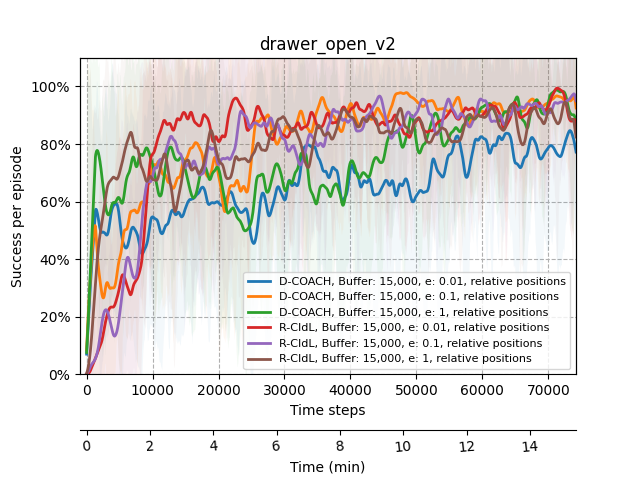
\includegraphics[width=0.5\textwidth]{figures/drawer_same_buffer_v2.png}\label{fig:drawer_open_same_e}}
   \hfill
  \subfloat{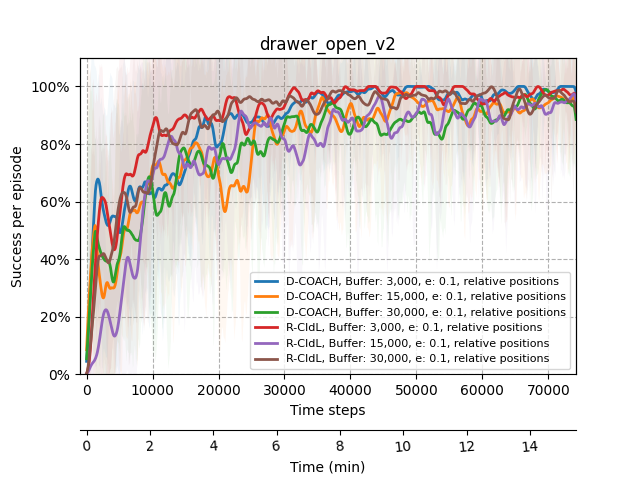
\includegraphics[width=0.5\textwidth]{figures/drawer_same_e_v2.png}\label{fig:drawer_open_same_buffer}}

  \caption{drawer-open-v2 results using a simulated teacher $P_h: \alpha = 0.9; \tau =  0.000015$. On the left, a comparison of the influence of the $e$ parameter on the baseline method D-COACH and on R-CIdL. On the right, a comparison of how different buffer sizes affect both methods.}
  \label{fig:results_drawer_open_buffer_e}
\end{figure}

From the previous analysis, the best combinations of buffer size $K$ and $e$ for both methods when positions are relative are $K=30000$ and $e=0.1$ for R-CIdL and $K=3000$ and $e=0.1$ for D-COACH. The experiments are repeated with the same values but this time considering absolute positions instead of relative ones. Figure \ref{fig:results_drawer_open_best}  shows this comparison where R-CIdL is able to reach similar levels of performance as in the case of relative positions. In the case of D-COACH, its performance soon reaches an average success of 70\% which increases just at the end of the training. Still, for D-COACH the difference in success between relative and absolute positions is remarkable.


\begin{figure}[H]
    \centering
    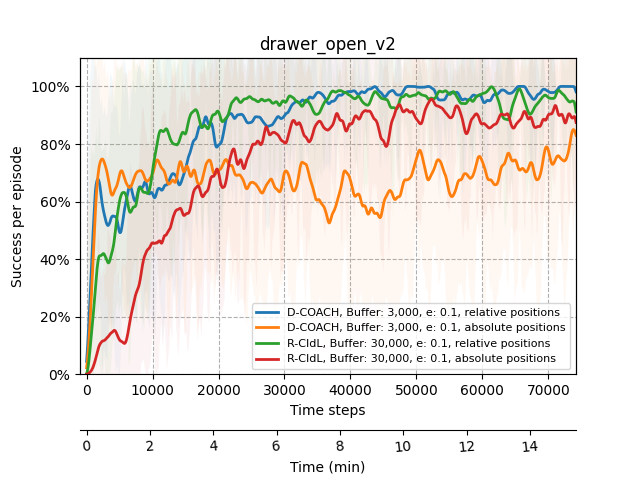
\includegraphics[width=.6\textwidth]{figures/drawer_best_v2.png}
    \caption{drawer\_open\_v2 results using a simulated teacher $P_h: \alpha = 0.9; \tau =  0.000015$. Comparison of the best performance of each method in relative positions, against their performances in absolute positions with the same conditions of buffer and $e$.}
    \label{fig:results_drawer_open_best}
\end{figure}


\section{Results of validation in real system}
\label{section:results_kuka}

To validate the proposed R-CIdL algorithm in a real system, we taught the 2 planar manipulation tasks described in sections \ref{subsection:Park a box} and \ref{subsection:Push box in a straight line}. The human teacher provided the necessary corrections to the position of the end effector with a joystick. In this subsection we show the results obtained for both tasks and because the objective is simply to validate R-CIdL, we did not performed comparisons with other methods. 


\subsection{Results for task "push a box"}
\label{subsection:results_kuka_push}
The result for the task "push a box" in figure \ref{fig:kukapush} shows the average success per episode of R-CIdL after a training of 60 minutes with a human teacher where 165 episodes were performed. Prior to the final training, some trials were done to adjust the value of $e$ which was found to work best with a value of 0.5. The replay buffer size $k$ for this task was set to 10000 which never got completely full because the human sends around 7300 correction signals.
The learning was evaluated every 5 episodes and every episode was on average 20 seconds long. At minute 23 approximately, the slope of the curve starts increasing until minute 35 when the success percentage reaches an average of 80\%.








% 165 episodes, evaluation every 5 episodes

% 7365 feedback signals
% Accumulated timesteps 13135
% e 0.5, buffer 10000 that never gets fully complete meaning that all the feedback provided is used to update the HumanModel
% Average timesteps per episode 72

% aprox 20 secs per episode

% at episode 60, 23 min the slope of the curve starts increasing until 130 episode (47 min) when the percentage of success is 80% aprox



\begin{figure}[H]
    \centering
    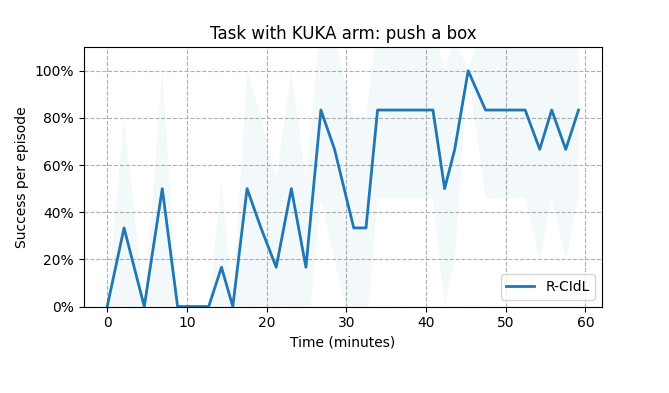
\includegraphics[width=.7\textwidth]{figures/push_1.png}
    \caption{Results of the task "push the box" with a human teacher.}
    \label{fig:kukapush}
\end{figure}

\subsection{Results for task "park a box"}
\label{subsection:results_kuka_park}

The results for the task "park a box" in figure \ref{fig:kukapark} show the average success per episode of R-CIdL after a training of 40 minutes with a human teacher where 65 episodes were performed. Prior to the final training, some trials were done to adjust the value of $e$ which was found to work best with a value of 0.3. The buffer size for this task was set to 10000 which never got completely full because the human sends around 3400 feedback signals.
The learning was evaluated every 5 episodes and every episode was on average 36 seconds long. Around minute 25 the performance increases drastically. This point in time corresponds with the moment that the R-CIdL agent learns to go around the corner (see third frame of figure \ref{fig:sequence-park-box}). Prior to that moment, all episodes logically fail. At episode 37, the performance reaches its maximum as all the following episodes are successful.



\begin{figure}[H]
    \centering
    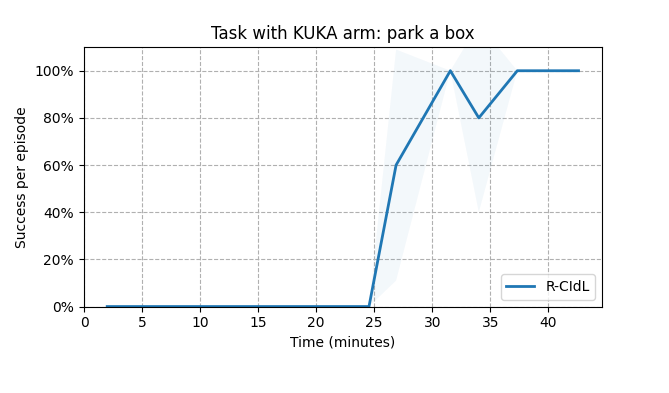
\includegraphics[width=.7\textwidth]{figures/park_1.png}
    \caption{Results of the task "park the box" with a human teacher.}
    \label{fig:kukapark}
\end{figure}